% Created 2017-04-17 Mon 16:27
\documentclass[11pt]{article}
\usepackage[utf8]{inputenc}
\usepackage[T1]{fontenc}
\usepackage{fixltx2e}
\usepackage{graphicx}
\usepackage{longtable}
\usepackage{float}
\usepackage{wrapfig}
\usepackage{rotating}
\usepackage[normalem]{ulem}
\usepackage{amsmath}
\usepackage{textcomp}
\usepackage{marvosym}
\usepackage{wasysym}
\usepackage{amssymb}
\usepackage{hyperref}
\tolerance=1000
\usepackage{color}
\usepackage{minted}
\usepackage{color}
\usepackage{minted}
\usepackage{parskip}
\author{Tammo Rukat}
\date{March 29, 2017}
\title{The OrMachine}
\hypersetup{
  pdfkeywords={},
  pdfsubject={},
  pdfcreator={Emacs 25.1.1 (Org mode 8.2.10)}}
\begin{document}

\maketitle
\setcounter{tocdepth}{1}
\tableofcontents


\section*{Introduction to Latent Variable Models}
\label{sec-1}
\subsection*{Notation and Graphical Model}
\label{sec-1-1}
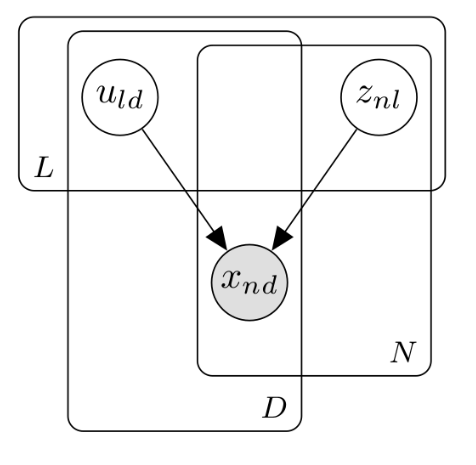
\includegraphics[width=.9\linewidth]{./plate_model.png}
\begin{itemize}
\item Mixture models
\item Factor Analysis (PCA)
\end{itemize}
\begin{itemize}
\item Variables
\begin{itemize}
\item ${x_{nd}}$ -- observations
\item ${u_{ld}}$ -- parameters (globale variables, weights)
\item ${z_{nl}}$ -- latent variables (local variables)
\end{itemize}
\item Indices
\begin{itemize}
\item ${n = 1\ldots N}$ -- observations/specimens
\item ${d = 1\ldots D}$ -- features (e.g. pixels or genes)
\item ${l = 1\ldots L}$ -- latent dimensions
\item ${k = 1\ldots K}$ -- layers
\end{itemize}
\item N observations
\item D features
\item L latent variables
\item K layers / abstraction levels
\end{itemize}

\subsection*{Neural network}
\label{sec-1-2}
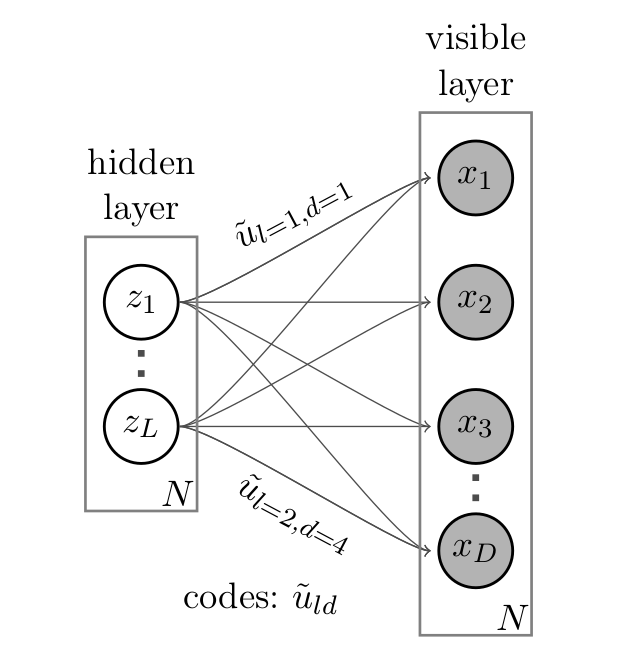
\includegraphics[width=.9\linewidth]{./single_layer_network.png}
\begin{itemize}
\item Major difference to feed forward neural nets: Nodes \textbf{and} weights are stochastic
\end{itemize}
\subsection*{What makes a good latent variable model for biological data?}
\label{sec-1-3}
\section*{The OrMachine}
\label{sec-2}
$$p(x_{nd}|\mathbf{u},\mathbf{z},\lambda)=
\sigma\left[ \lambda \right]\;\text{if}\;x=\min(1,\mathbf{u}_d^T\mathbf{z}_n)\;\text{else}:\;1-\sigma\left[ \lambda \right] \\
 = \sigma\left[\lambda \tilde{x}_{nd} (1-2\prod\limits_{l}(1-z_{nl}u_{ld}) \right]$$
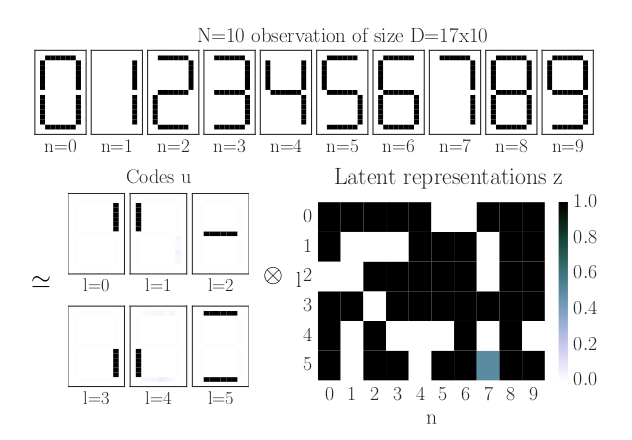
\includegraphics[width=.9\linewidth]{./calc_digit_intro.png}
\subsection*{Dispersion paramter $\lambda$}
\label{sec-2-1}
\begin{itemize}
\item Introducing a count variable $P$, that counts how many entries $x_{nd}$ are correctly predicted by the deterministic model $$ P = \sum\limits_{n,d} I\left[x_{nd}=(1-2\prod\limits_{l}(1-z_{nl}u_{ld})\right] $$
\item We can rewrite the likelihood
$$ L = \sigma(\lambda)^P \sigma(-\lambda)^{(ND-P)} $$
\item We find the maximum likelihood estimate of $\sigma(\lambda)$ as the fraction of entries that is aligned with the model prediction:
\end{itemize}
$$ \sigma(\lambda)_{\text{mle}} =\frac{P}{ND}\;. $$
\subsection*{Multi-layer OrMachine}
\label{sec-2-2}
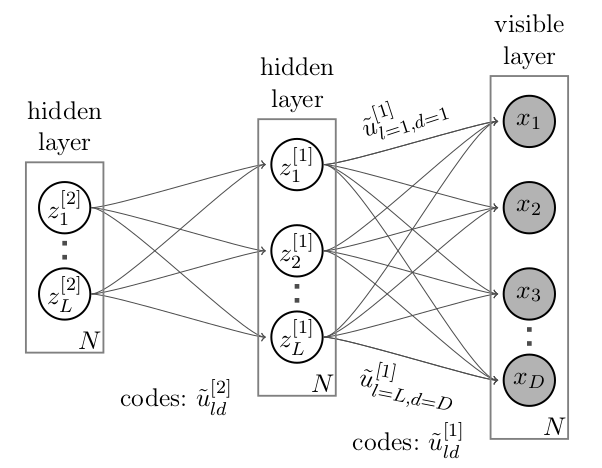
\includegraphics[width=.9\linewidth]{./twolayer_hm.png}

With ${\mathbf{z}^{[0]}_n = \mathbf{x}_n}$ and ${L^{[0]} = D}$, that is
$$  p(\mathbf{Z}^{[0:K]},\mathbf{U}^{[1:K]},\lambda) = 
  p(\mathbf{Z}^{[K]}) \prod_{k=0}^{K-1} p(\mathbf{Z}^{[k]}|\mathbf{Z}^{[k{+}1]},\mathbf{U}^{[k{+}1]},\lambda^{[k{+}1]})\, p(\mathbf{U}^{[k{+}1]})\, p(\lambda^{[k{+}1]}) 
$$

The joint density factorises in terms of the form p(layer|parents)

\section*{Inference for the OrMachine}
\label{sec-3}
\subsection*{Full conditionals}
\label{sec-3-1}
\begin{itemize}
\item Likelihood $$L = \sigma\left[\lambda \tilde{x}_{nd} (1-2\prod\limits_{l}(1-z_{nl}u_{ld}) \right]$$
\item Conditional for $z_{nl}$ $$ p(z_{nl}|\text{rest}) = \sigma\left[\lambda \tilde{z}_{nl} \sum\limits_d \tilde{x}_{nd}\; u_{ld}\prod\limits_{l^*\neq l} (1-z_{nl^*}u_{l^*d})\right] $$
\item Fast computation: One criterium fullfilled $\rightarrow$ the value of the term inside the sum over $d$ is known without considering its remaining terms.
\begin{itemize}
\item $u_{ld} = 0$. The effect of $z_{nl}$ on the likelihood  absent if $u_{ld}=0$.
\item $z_{nl^*}u_{l^*d} = 1$ for $l^* \neq l$. Another parent of $x_{nd}$ is already 1. Any additional parents will have no effect.
\end{itemize}
\end{itemize}
\subsection*{Implementation}
\label{sec-3-2}
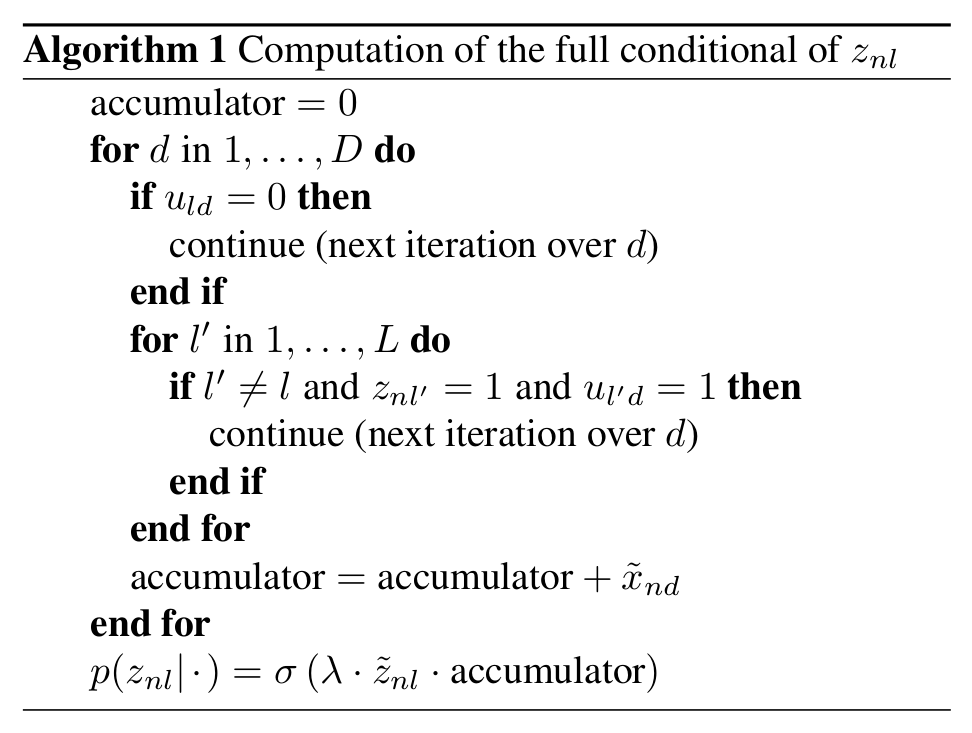
\includegraphics[width=.9\linewidth]{./alg1_2.png}
\subsection*{A modified binary state Gibbs sampler}
\label{sec-3-3}
\begin{itemize}
\item Discrete variables. New state $\mathbf{y}$, old state $\mathbf{x}$.
\item In a Gibbs sampler we draw a new value $y_i$ from $$ \pi(y_i|x_{-i}) $$
\begin{itemize}
\item The Metropolis Hasting acceptance probability is always 1. $$ $$
\end{itemize}
\item In the modified sampler we draw a new  $y_i$, \textbf{different from the old value} $x_i$ with probability $$ 1 = \frac{\pi(y_i|x_{-i})}{1-\pi(x_i|x_{-i})}\;. $$
\begin{itemize}
\item Acceptance probability = mutation probability: $$\alpha=\frac{\pi(y_i|x_{-i})}{\pi(x_i|x_{-i})(y_i,x_i)} = \frac{\pi(y_i|x_{-i})}{1-\pi(y_i|x_{-i})} $$
\end{itemize}
\item Off diagonal elements of the transition matrix:
$$  \frac{\pi(y_i|x_{-i})}{1-\pi(y_i|x_{-i})} \ge \pi(y_i|x_{-i}) $$
\end{itemize}
\subsection*{Metropolised Gibbs sampler - Algorithm}
\label{sec-3-4}
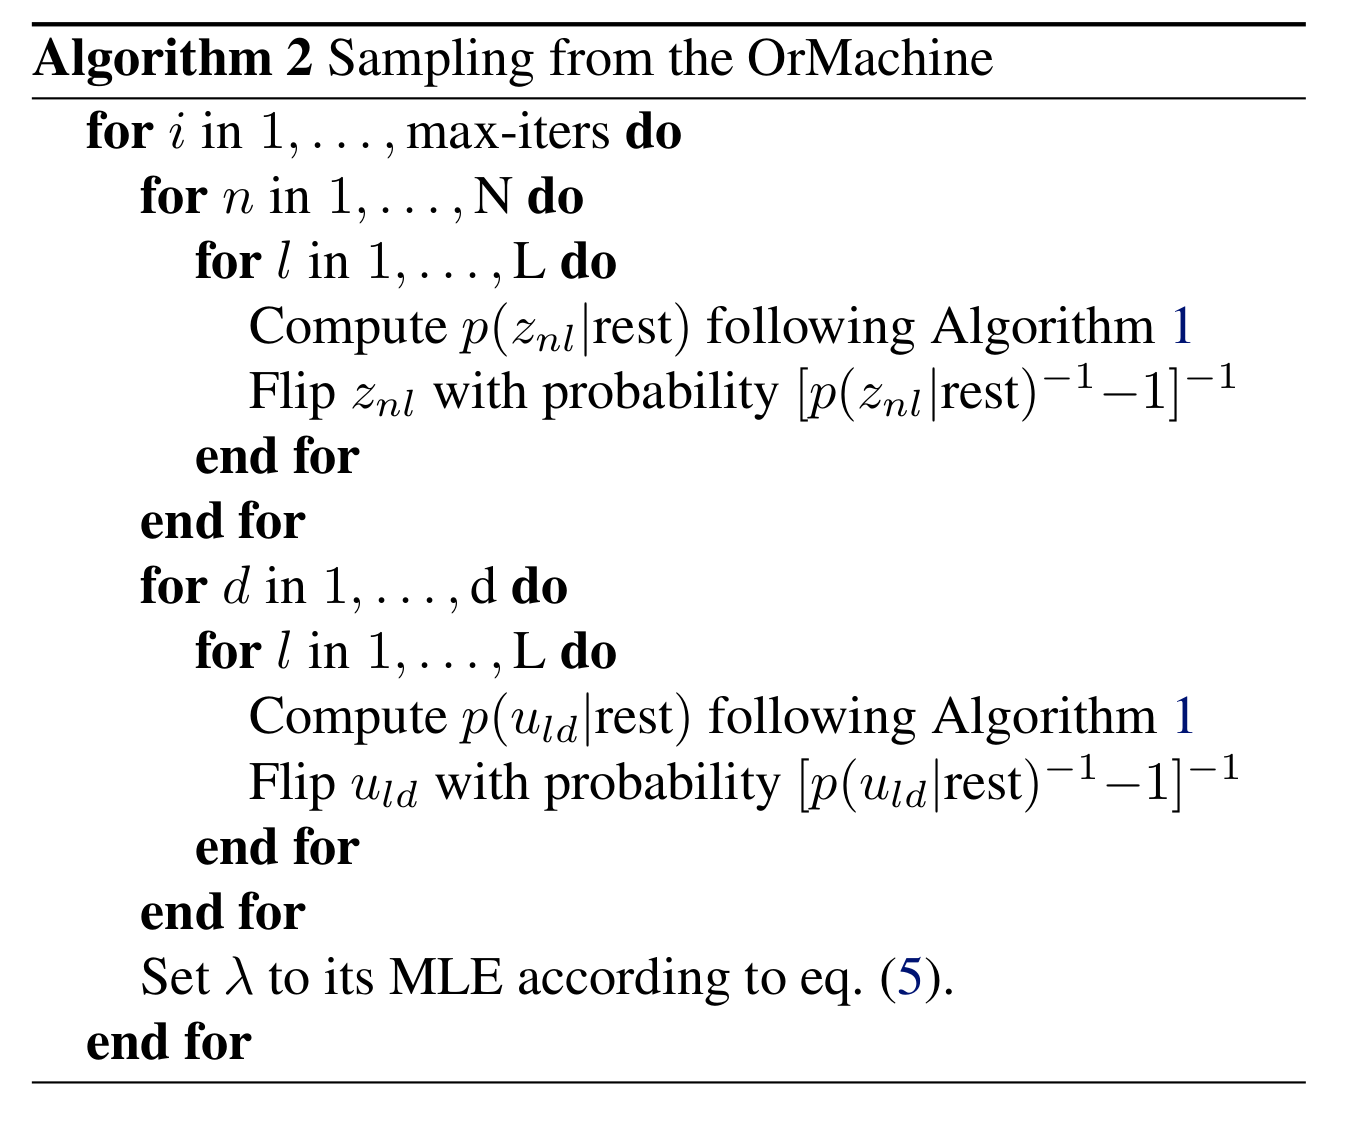
\includegraphics[width=.9\linewidth]{./alg2.png}
\subsection*{Speed}
\label{sec-3-5}
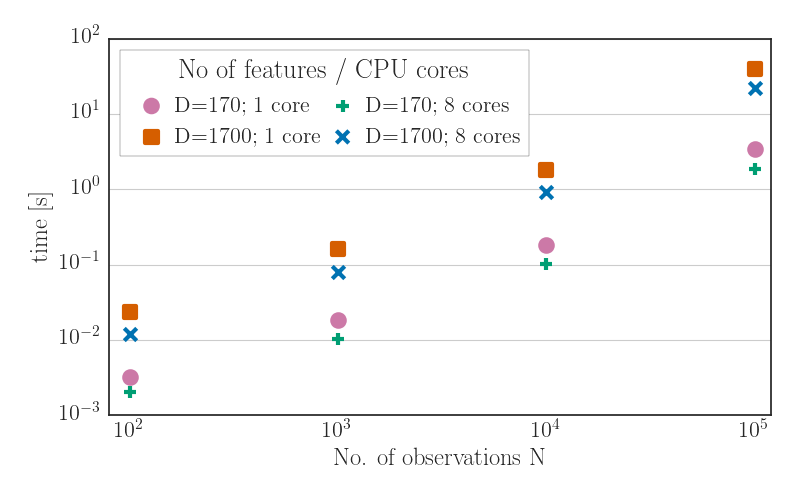
\includegraphics[width=.9\linewidth]{./scaling_parallel.png}
\section*{Examples and Experiments}
\label{sec-4}
\subsection*{Random matrix factorisation}
\label{sec-4-1}
\subsubsection*{Problem setting}
\label{sec-4-1-1}
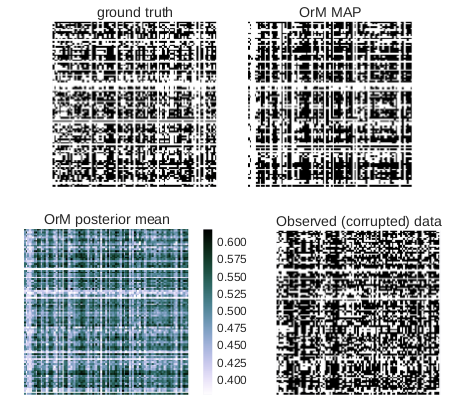
\includegraphics[width=.9\linewidth]{./factorisation.png}
\subsubsection*{Performance}
\label{sec-4-1-2}
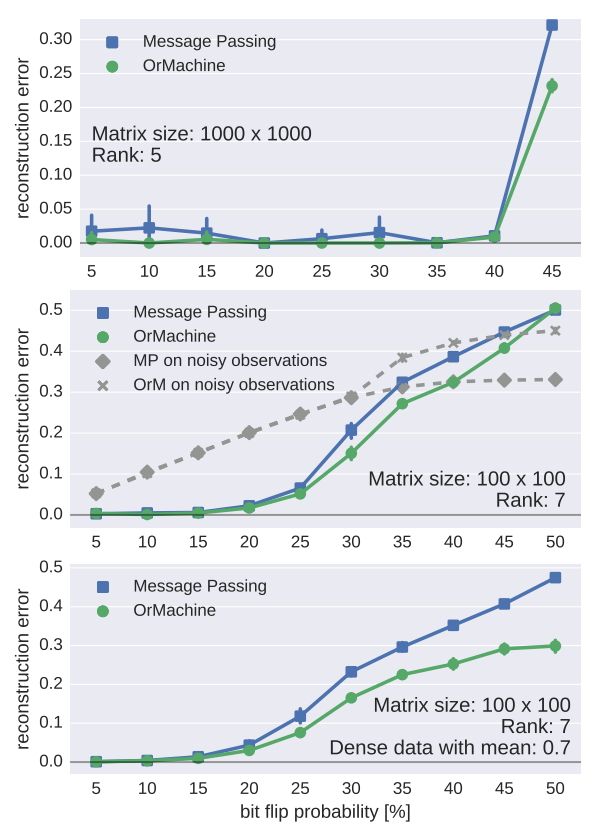
\includegraphics[width=.9\linewidth]{./factorsiation_performance_new.png}
\subsection*{Random matrix completion}
\label{sec-4-2}
\begin{itemize}
\item Remember likelihood and conditionals: $$L = \sigma\left[\lambda \tilde{x}_{nd} (1-2\prod\limits_{l}(1-z_{nl}u_{ld}) \right]$$ $$ p(z_{nl}|\text{rest}) = \sigma\left[\lambda \tilde{z}_{nl} \sum\limits_d \tilde{x}_{nd}\; u_{ld}\prod\limits_{l^*\neq l} (1-z_{nl^*}u_{l^*d})\right] $$
\item Set an unobserved observation to $x_{nd} = 0.5 \;\rightarrow\; \tilde{x}_{nd}=0$
\end{itemize}
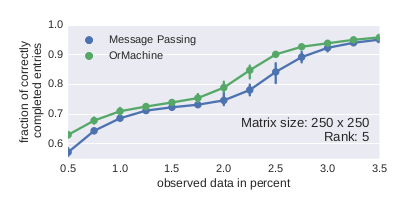
\includegraphics[width=.9\linewidth]{./completion1.png}
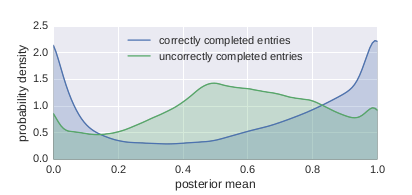
\includegraphics[width=.9\linewidth]{./completion2.png}
\subsection*{MovieLense}
\label{sec-4-3}
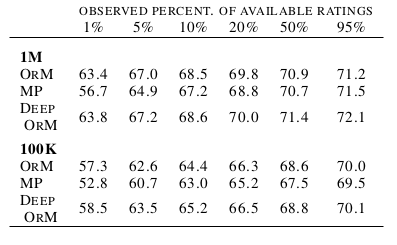
\includegraphics[width=.9\linewidth]{./movielense1.png}
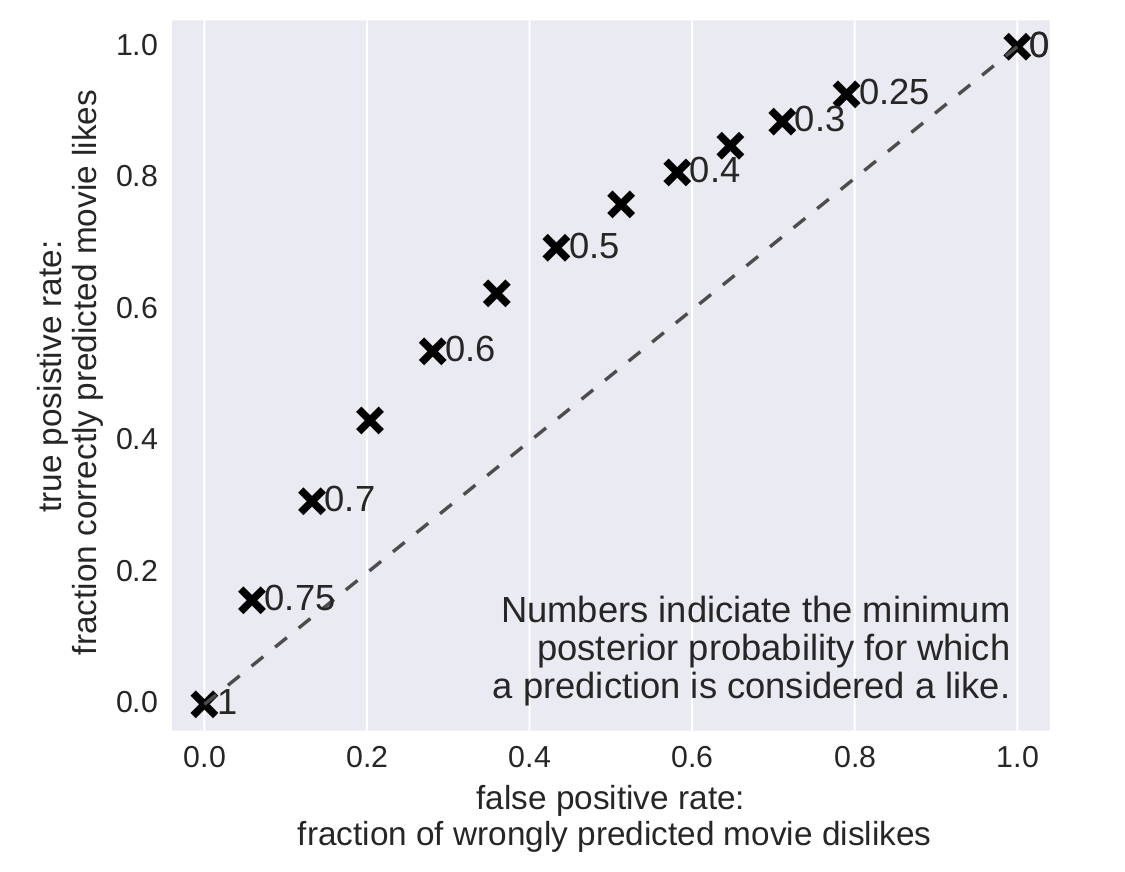
\includegraphics[width=.9\linewidth]{./ml_roc.png}
\subsection*{Calculator digits}
\label{sec-4-4}
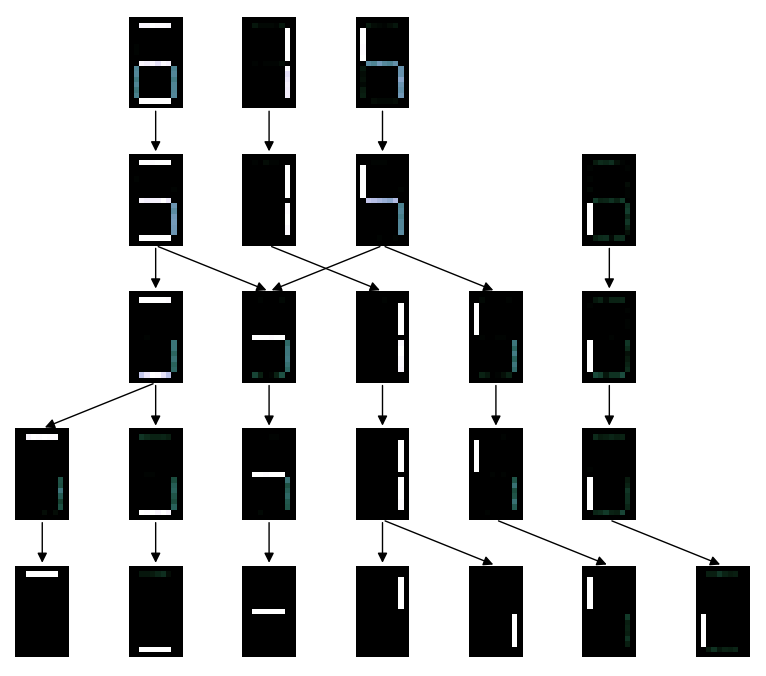
\includegraphics[width=.9\linewidth]{./calc_hierarchy.png}
\subsubsection*{MNIST}
\label{sec-4-4-1}
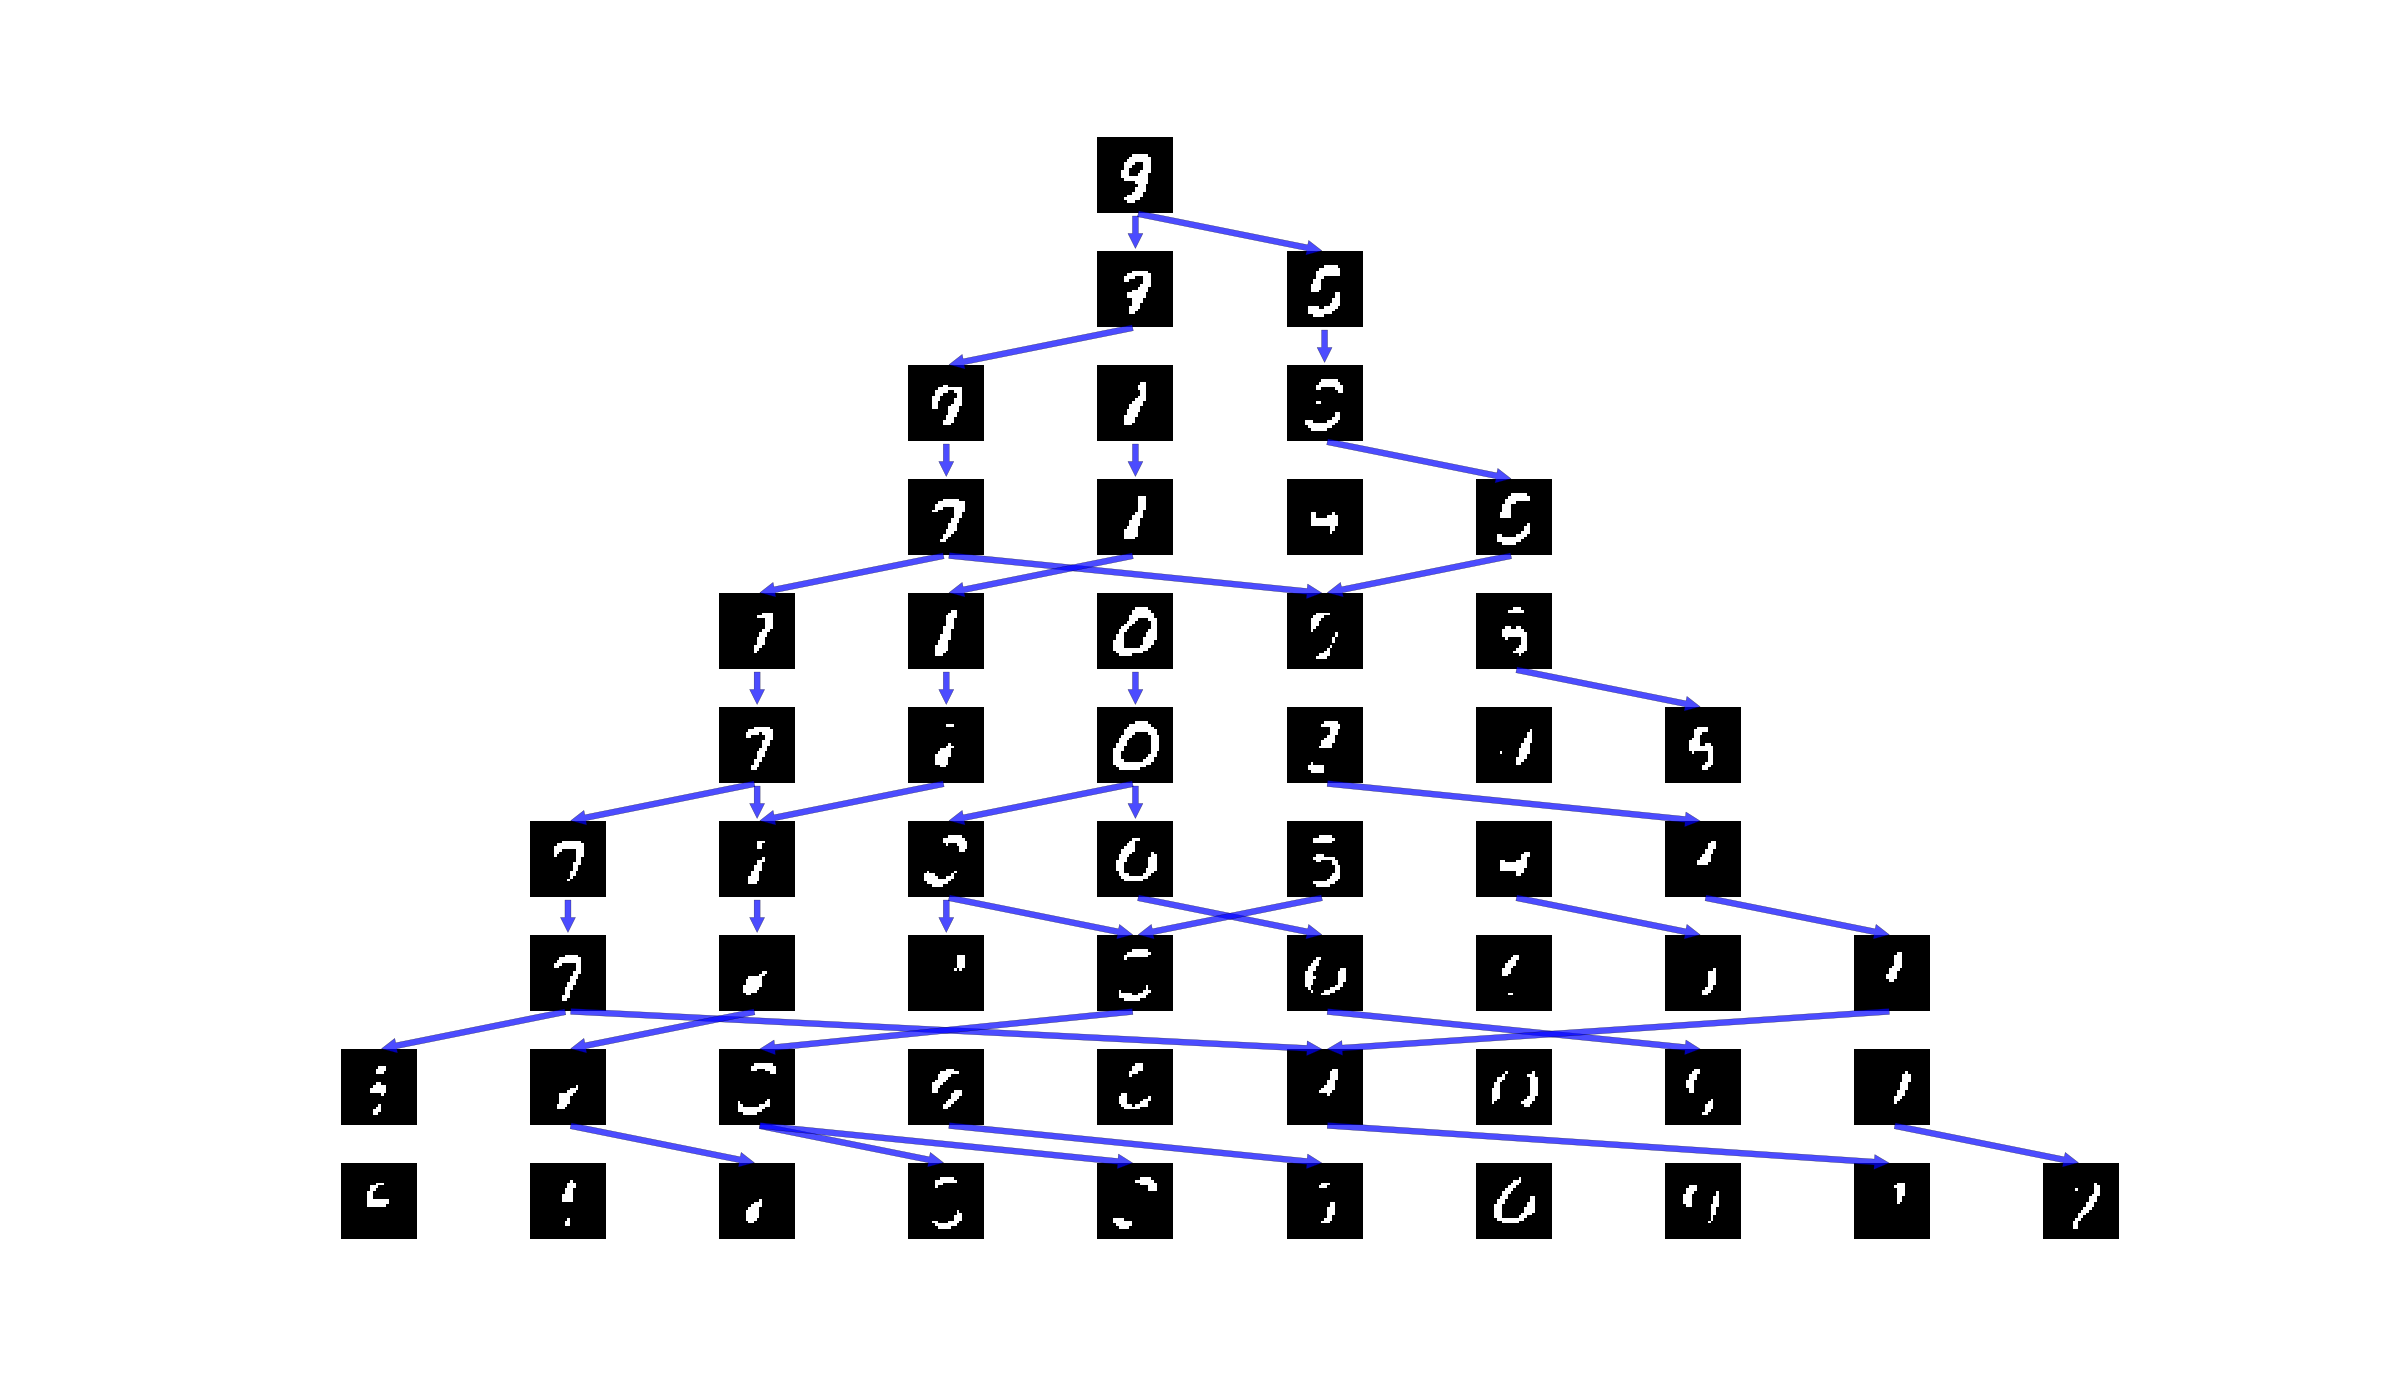
\includegraphics[width=.9\linewidth]{./mnist_hierarchy.png}
\subsection*{Single cell data I}
\label{sec-4-5}
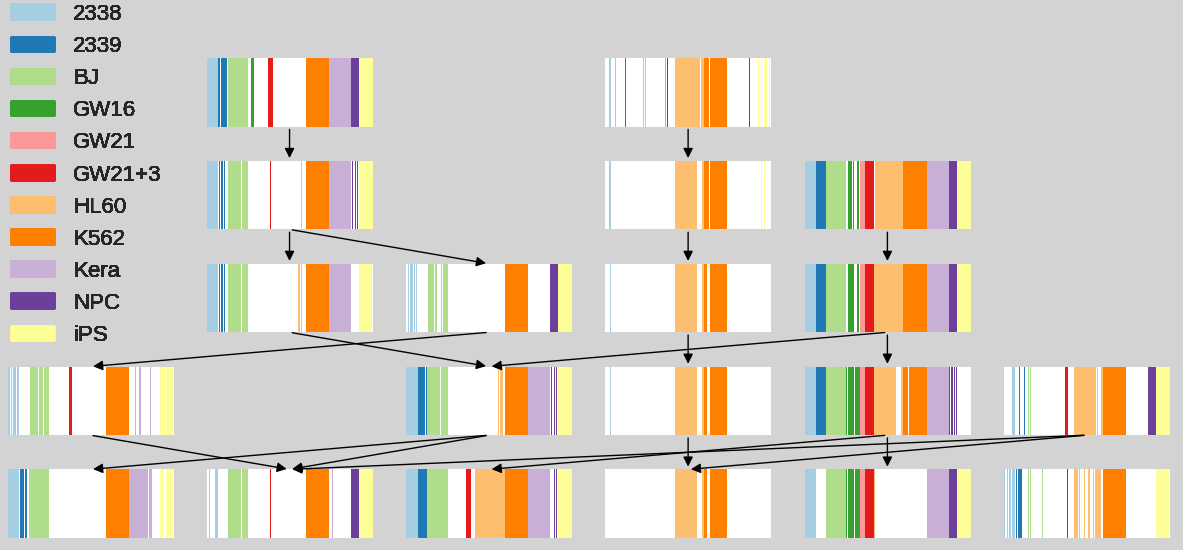
\includegraphics[width=.9\linewidth]{./sc_hierarchy.png}
\subsection*{Single cell data II - 1.3 Million Brain Cells from E18 Mice}
\label{sec-4-6}
\subsubsection*{Gene patterns}
\label{sec-4-6-1}
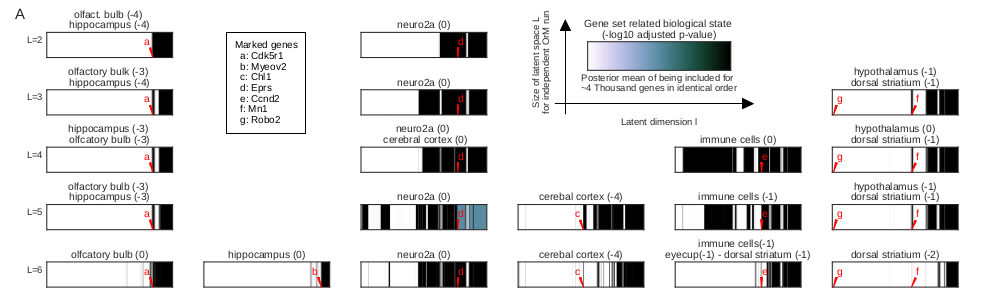
\includegraphics[width=.9\linewidth]{./mice_neurons1.png}
\subsubsection*{Specimen representations}
\label{sec-4-6-2}
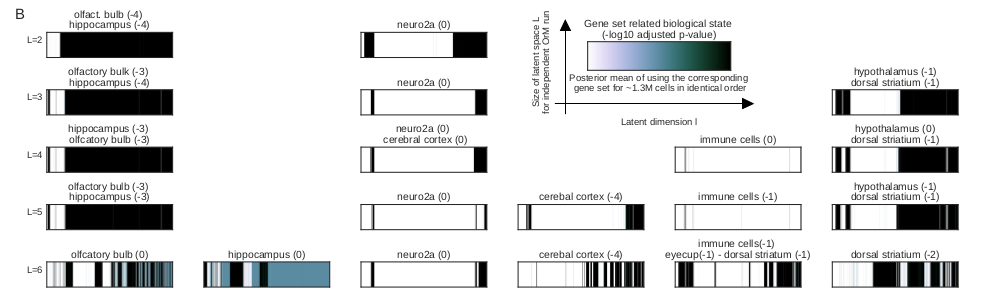
\includegraphics[width=.9\linewidth]{./mice_neurons2.png}
\subsection*{Deep calculator digits}
\label{sec-4-7}
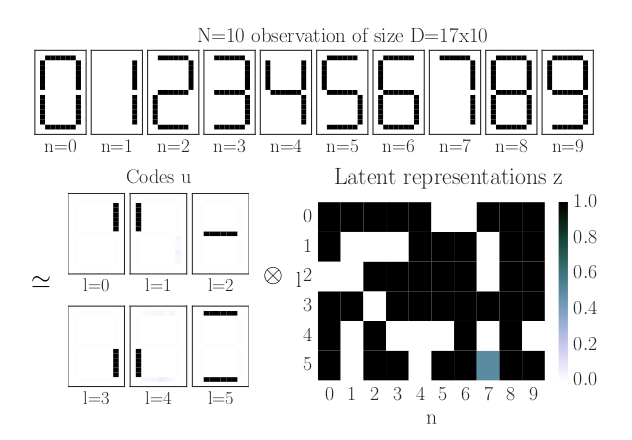
\includegraphics[width=.9\linewidth]{./calc_digit_intro.png}
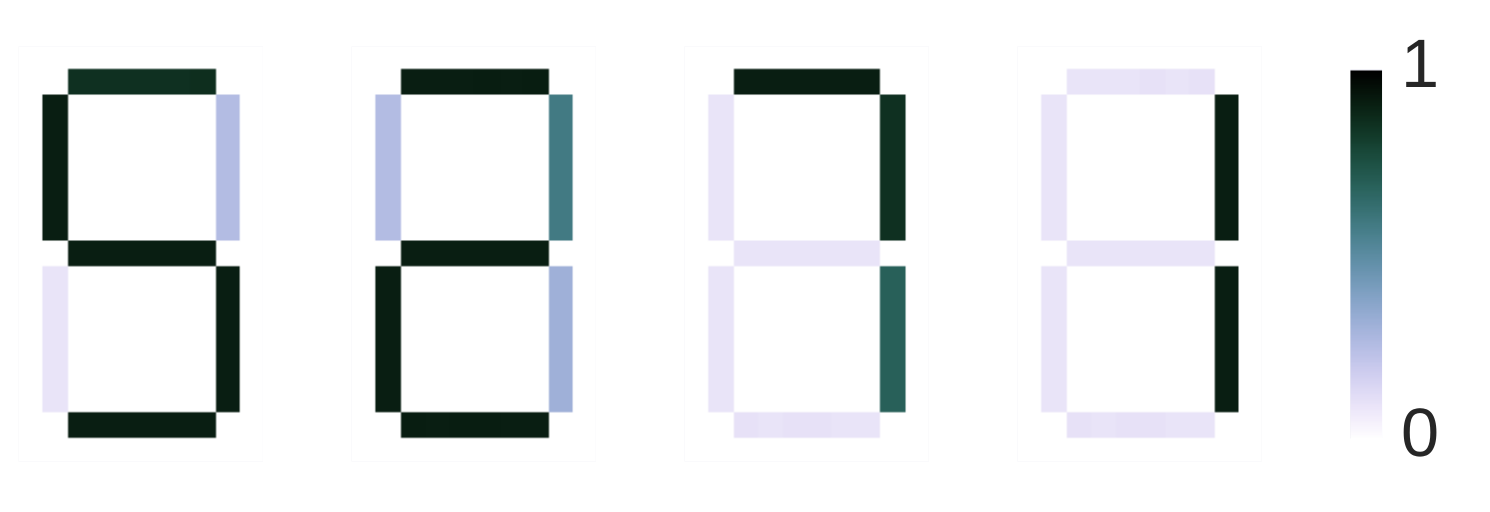
\includegraphics[width=.9\linewidth]{./deep_calc.png}
\begin{itemize}
\item Second layer representation fed forward to data layer.
\end{itemize}
\subsection*{Deep noisy calculator digits}
\label{sec-4-8}
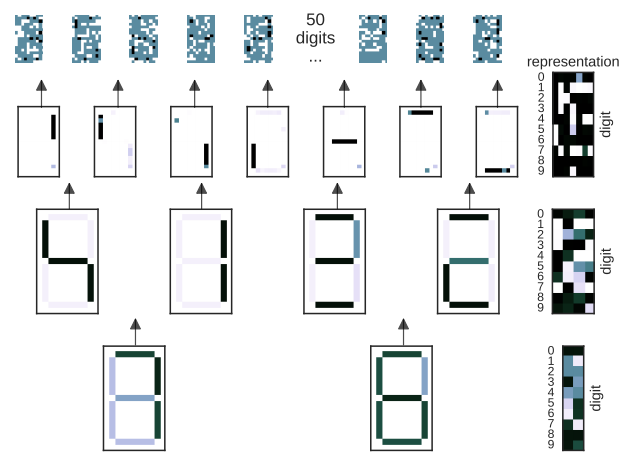
\includegraphics[width=.9\linewidth]{./deeper_calc.png}
\begin{itemize}
\item Input: 50 digits with 70\% missing observations
\item Reducde reconstruction error from 1.4\% to 0.4\% compared to shallow model
\end{itemize}
\subsection*{Pancan and pathway data}
\label{sec-4-9}
\subsubsection*{Setup}
\label{sec-4-9-1}
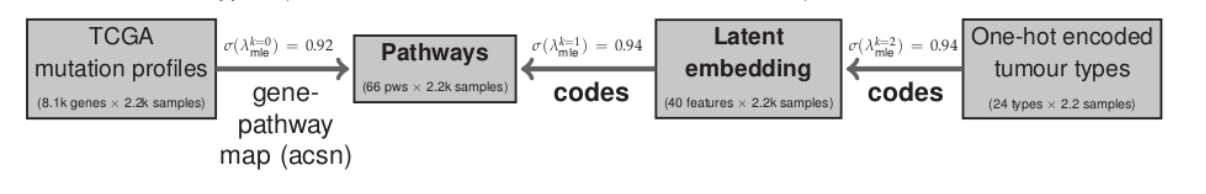
\includegraphics[width=.9\linewidth]{./arc.png}
\subsubsection*{"Data"}
\label{sec-4-9-2}
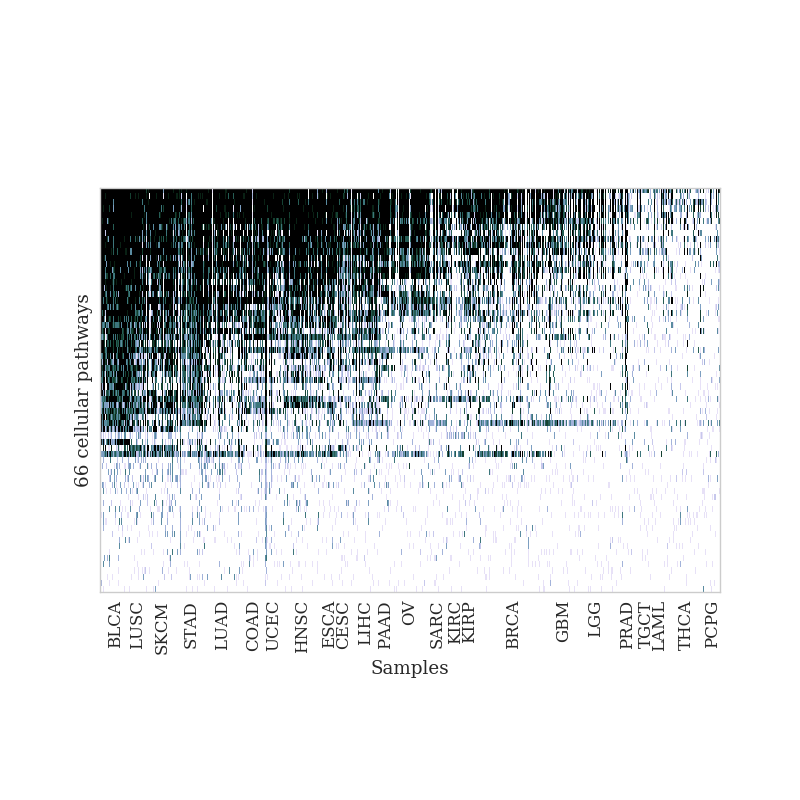
\includegraphics[width=.9\linewidth]{./fa_data_prob.png}
\subsubsection*{Embedding}
\label{sec-4-9-3}
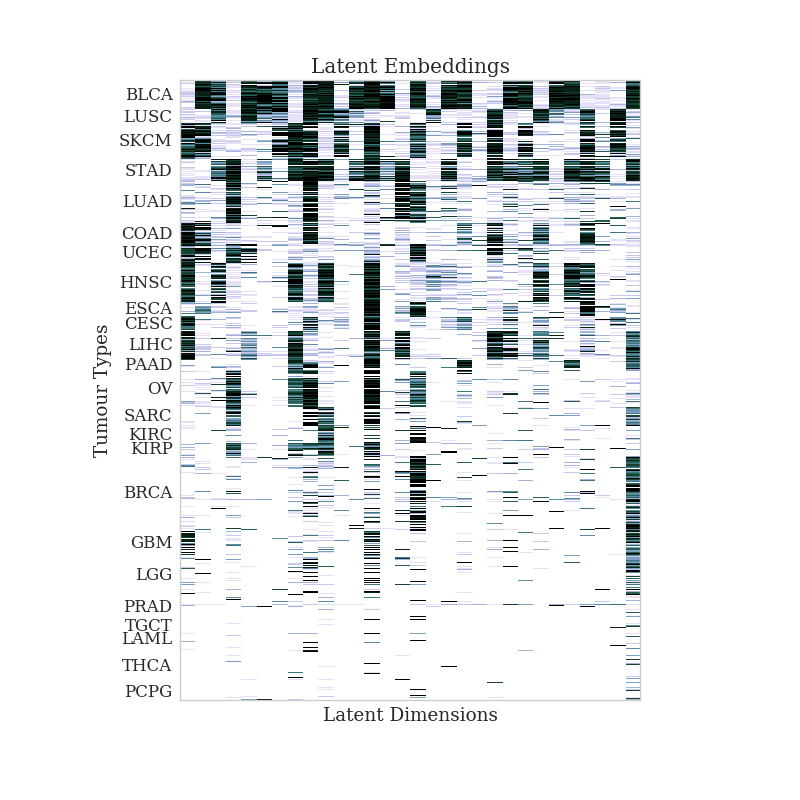
\includegraphics[width=.9\linewidth]{./fa_pw_latent.png}
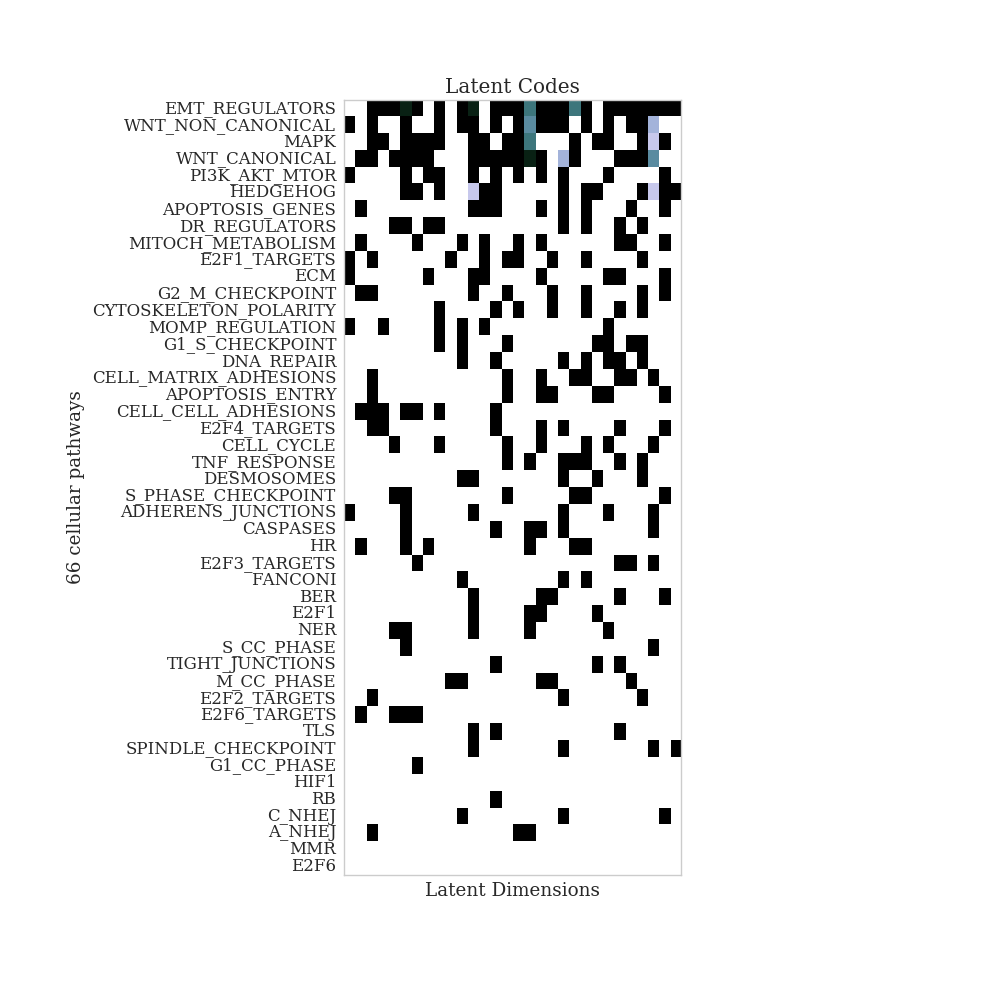
\includegraphics[width=.9\linewidth]{./fa_pw_patterns.png}
\subsubsection*{Predictive}
\label{sec-4-9-4}
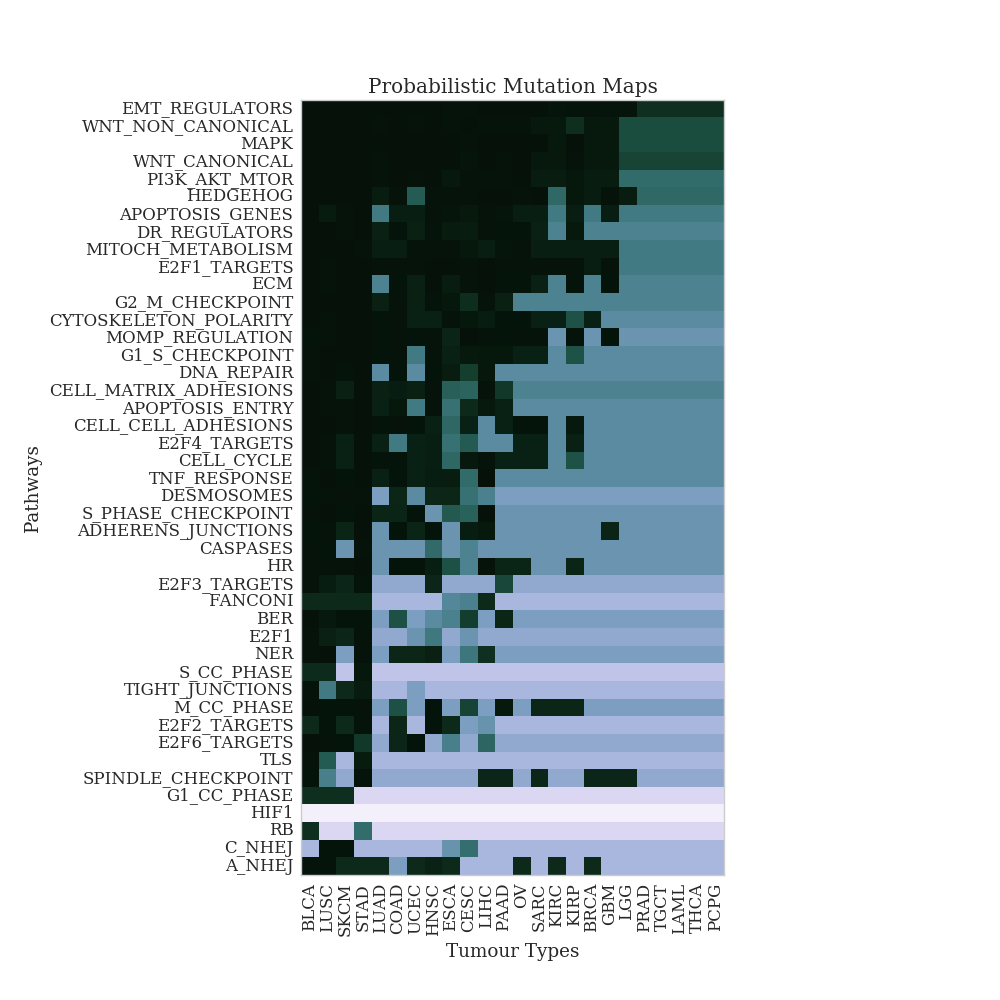
\includegraphics[width=.9\linewidth]{./fa_pw_predictive.png}
\section*{Additional Material}
\label{sec-5}
\subsection*{Preprint on ArXiv}
\label{sec-5-1}

\includegraphics[width=.9\linewidth]{./arxiv.png}
\subsection*{Hamming Machine}
\label{sec-5-2}
\begin{itemize}
\item Construct a probability distribution based on the hamming distance between two binary vectors, ${h(\mathbf{x},\mathbf{u})}$, and a dispersion parameter ${\lambda}$: $$ p(\mathbf{x}|\mathbf{u}) \propto \exp\left[ -\lambda \, h(\mathbf{x},\mathbf{u}) \right] $$
\item Each observations ${\mathbf{x} }$ is generated from a subset of binary \textbf{codes}: ${\mathbf{u}_{l{=}1\ldots L}}$, selected by a vector of binary latent variables ${\mathbf{z}}$ $$ p(\mathbf{x}|\mathbf{U},\mathbf{z},\lambda) \propto \prod\limits_l p(\mathbf{x}|\mathbf{u}_l,\lambda)^{z_l} = \prod\limits_d \exp\left[- \sum_l z_l \lambda h(x_d,u_{ld}) \right]$$
\item Normalising the likelihood for for binary observations yields a \textbf{logistic sigmoid}: $$ p(x_d = 1|\mathbf{z}, \mathbf{u}_{1\ldots L}, \lambda) = \frac{1}{1+\exp\left[-\lambda \sum\limits_l z_l (2u_{ld} - 1) \right]} = \sigma\left[\lambda \sum_l z_l \tilde{u}_{ld} \right]$$
\item We defined the mapping from ${\{0,1\}}$ to ${\{{-}1,1\}\,}$: $\;\;{\tilde{u} = 2u{-}1}$
\end{itemize}
\subsection*{One-hot sampling}
\label{sec-5-3}
% Emacs 25.1.1 (Org mode 8.2.10)
\end{document}